\chapter{Introduction}\label{C:intro}

This proposal presents the use of permutation entropy and ordinal patterns in time series analysis, including the calculation of pattern histograms, entropy, and complexity to better understand their statistical properties. Additionally, the confidence intervals for entropy and complexity under the multinormal distribution and features for time series clustering are discussed. The concept of ordinal patterns in time series was introduced by Bandt and Pompe \cite{PhysRevLett.88.174102}. This study focuses on features derived from Bandt \& Pompe symbolization, specifically Shannon entropy. Future work will extend to other measures, such as Rényi entropy, Fisher information, and the confidence intervals for their entropy and complexity under the multinormal distribution. Features for time series clustering within ordinal patterns for time series analysis will be further studied.

Time series analysis is widely applied across various fields, including engineering, economics, physical sciences, and more. A time series is defined as a collection of observations ${x_t}$, each representing a realized value of a particular random variable $X_t$, where time can be either discrete or continuous.

Examples of time series applications include finance (e.g., analyzing exchange rate movements or commodity prices), biology (e.g., modeling the growth and decline of bacterial populations), medicine (e.g., tracking the spread of diseases like COVID-19 or influenza), and geoscience (e.g., predicting wet or dry days based on past weather conditions).

The primary goal of time series analysis is to understand the nature of the phenomenon represented by the observed sequence. Time domain and frequency domain methods are the two primary approaches used in time series analysis. The temporal approach relies on concepts such as auto-correlation and regressions, where a time series' present value is analyzed in relation to its own past values or the past values of other series. This method represents time series directly as a function of time. On the other hand, the spectral approach represents time series through spectral expansions, such as wavelets or Fourier modes \cite{treitel1995spectral}. 
%%% ACF Spectral, temporal or both? Citation 
However, these methods often require assumptions such as large sample sizes or normally distributed observations that are rarely met in real-world empirical data. For many statistical techniques to be valid, these assumptions must hold, but in practice, they are frequently violated.
%%% ACF The problems of traditional approaches should be discussed before non-parametric techniques
For example, traditional approaches to time series analysis, such as time domain and frequency domain methods, rely on assumptions that are not always valid in real-world data. The time domain approach, which uses techniques like auto-correlation and regression, assumes stationarity and often struggles with nonlinear or nonstationary data. Similarly, the frequency domain approach, which represents time series through spectral expansions such as wavelets or Fourier modes, may require assumptions about periodicity and may not effectively capture short-term fluctuations.

Many statistical methods in these approaches depend on specific conditions, such as large sample sizes or normally distributed observations. However, these assumptions are often unrealistic, leading to inaccurate or biased results. When such conditions are not met, alternative methods must be considered.

As a result, alternative methods, often referred to as non-parametric techniques, must be considered. These methods rely on the rank $R_t$ of the observations $x_t$ rather than their actual values, making them robust and applicable to a wide range of data sets. Since non-parametric tests do not assume a normal distribution, they are highly reliable. For example, the Kruskal-Wallis $H$ test and the Wilcoxon test are effective tools for comparing two or more population probability distributions from independent random samples. However, these techniques are not always suitable for time series data, which often require specialized methods tailored to their unique characteristics.

To address these challenges, ordinal pattern methods provide a robust alternative. Instead of analyzing the absolute values of a time series, these methods focus on the order relationships between consecutive data points. This approach effectively captures the underlying dynamics of complex systems and offers several advantages.

The ordinal pattern-based method has become a widely used tool for characterizing complex time series. Since its introduction nearly twenty-three years ago by Bandt and Pompe in their foundational paper \cite{PhysRevLett.88.174102}, it has been successfully applied across various scientific fields, including biomedical signal processing, optical chaos, hydrology, geophysics, econophysics, engineering, and biometrics. It has also been used in the characterization of pseudo-random number generators.
   
%%% ACF Give a broader context and application. Machine diagnosis is just your starting point
The method proposed by Bandt and Pompe has been highly successful in analyzing time series. They computed Shannon entropy from the histogram of causal patterns by transforming the time series into ordinal patterns while preserving the original data structure. The histogram is then constructed based on these patterns.

This approach offers several advantages. The resulting distribution is less sensitive to outliers, and the histogram does not depend on any predefined model. These properties make ordinal patterns a valuable and practical tool for time series analysis, especially when traditional methods prove inadequate. Additionally, this method can effectively identify chaotic components within a sequence of words.

Later, Rosso \cite{Rosso2007} introduced an additional dimension to this analysis—Statistical Complexity—derived from the same histogram of causal patterns.

\section*{Introduction to Ordinal Pattern Analysis}

%%% ACF Rewrite this as an introduction to ordinal pattern analysis
Ordinal patterns are derived from non-parametric time series data rather than relying on their actual values. Ordinal patterns are transformations that encode the sorting characteristics of values in $\mathbb{R^D}$ into $D!$ symbols.One of the possible encoding is the set of indexes that sort the $D$ values in non-decreasing order, where $D$ is called the "Embedding Dimension" and usually ranges between three to six.  To illustrate this idea, let $X=\{x_1,x_2, \dots, x_{(n+D-1)}\}$ be a real valued time series of length $n+D-1$ without ties. As stated by Bandt \& Pompe, if the $\{x_t\}_{t=1}^{n+D-1}$ takes infinitely many values, it is common to replace them with a symbol sequence $\{{\pi}_j\}$ consisting of finitely many symbols and then compute the entropy from this sequence. The corresponding symbol sequence naturally emerges from the time series without requiring any model assumptions. We compute $\mathbf{{\pi}}=({\pi}_1, {\pi}_2,\dots, {\pi}_n)$ symbols from sub-sequences of embedding dimension $D$. There are $D!$ possible symbols: $\pi_j \in \mathbf{{\pi}}=({\pi}^1, {\pi}^2,\dots, {\pi}^{D!})$. The histogram of proportions $h=(h_1,h_2,\dots, h_{D!})$ in which the bin $h_l$ is the proportion of symbols of type $\pi^l$ of the total number of symbols. For our convenient, we will model those symbols as a $k$ dimensional ransom vector where $k=D!$.

Consider a series of $n$ independent trials in which only one of $k$ mutually exclusive events ${\pi}^1, {\pi}^2,\dots, {\pi}^k$ is observed with probability $p_1, p_2, \dots, p_k,$ respectively, where $p_l \geq 0$ and $\sum_{l=1}^{k} p_l=1.$ Suppose that $N=(N_1, N_2, \dots, N_k)$ is the vector of random variables that, with $\sum_{l=1}^{k} N_l=n$, counts how many times the events ${\pi}^1, {\pi}^2,\dots, {\pi}^k$ occur in the $n$ trials. Then, the joint probability distribution of $N$ is
\begin{equation}
	Pr(N=(n_1,n_2,\dots, n_k))=n!\prod_{l=1}^{k} \frac{p_l^{n_l}}{n_l !}
\end{equation}    
where $n_l \geq 0$ and $\sum_{l=1}^{k} n_l=n$ 
%%% ACF Rephrase
%%% ACF Use \dots


\section*{Problem Statement}
%To illustrate this concept, we consider food preferences among individuals as an example of time series data. Meal choices vary widely among people, reflecting their unique tastes and priorities. For instance, when selecting main meals such as beef, pork, chicken, fish, and vegetables, each person has distinct preferences. By analyzing these choices, we can uncover intriguing patterns that highlight the diversity in individual selections.

To illustrate this concept, imagine tracking the mean monthly humidity in Wellington. We want to analyze how humidity changes throughout the year. By examining this data, you can uncover interesting patterns that highlight the variations in humidity across different months. 

%Imagine two individuals with different meal preferences. Person 1 enjoys pork the most, followed by beef, fish, chicken, and vegetables. In contrast, Person 2 prefers chicken first, followed by fish, vegetables, beef, and pork. A simple graph illustrating these preferences would show that their choices do not overlap significantly, emphasizing their unique tastes.

%Expanding this analysis to a larger group allows us to observe even more diverse and complex patterns. Each individual's preference forms a unique data point, and collectively, they create a rich tapestry of variation. This exploration provides valuable insights into how food choices differ across individuals and groups, making the study both meaningful and captivating.

\begin{table}[ht]
	\caption{Mean monthly humidity variations in Wellington throughout the year} % title of Table
	\centering % used for centering table
	\begin{tabular}{c c } % centered columns (4 columns)
		\hline\hline %inserts double horizontal lines
		Month & Mean of relative humidity \\ [0.5ex] % inserts table
		%heading
		\hline % inserts single horizontal line
		January & 77.3 \\ % inserting body of the table
		February & 81 \\
		March & 82.4 \\
		April & 81.7 \\
		May & 83.6 \\ 
		June & 85.6 \\
		July & 84.4 \\
		August & 83.1 \\ 
		September & 78.8 \\
		October & 79.6 \\
		November & 78.2 \\
		December & 78.8 \\ [1ex] % [1ex] adds vertical space
		\hline %inserts single line
	\end{tabular}
	\label{table:nonlin} % is used to refer this table in the text
\end{table}

We can convert this actual data into ordinal patterns. To do this, for each month, we determine the order of the humidity values rather than their actual magnitudes. Each three-time-point sequence (which can be adjusted based on preference) is converted into an ordinal pattern. The sequence length can vary from 3 to 6 or more.

\begin{table}[ht]
	\caption{Ordinal Patterns} % title of Table
	\centering % used for centering table
	\begin{tabular}{c c	c } % centered columns (4 columns)
		\hline\hline %inserts double horizontal lines
		\# of patterns & Mean Humidity sequence & Ordinal Patterns \\ [0.5ex] % inserts table
		%heading
		\hline % inserts single horizontal line
		1 & (77.3,81,82.4) & (123) $=\pi_1$\\ 
		2 & (81,82.4,81.7) & (132) $=\pi_2$\\
		3 & (82.4,81.7,83.6) & (213) $=\pi_3$\\
		4 & (81.7,83.6,85.6) & (123) $=\pi_4$ \\
		5 & (83.6,85.6,84.4) & (132) $=\pi_5$\\ 
		6 & (85.6,84.4,83.1) & (321) $=\pi_6$\\
		7 & (84.4,83.1,78.8) & (321) $=\pi_7$\\
		8 & (83.1,78.8,79.6) & (312) $=\pi_8$\\ 
		9 & (78.8,79.6,78.2) & (231) $=\pi_9$\\
		10 & (79.6,78.2,78.8) & (312) $=\pi_{10}$\\ [1ex] % [1ex] adds vertical space
		\hline %inserts single line
	\end{tabular}
	\label{table:nonlin} % is used to refer this table in the text
\end{table}

In this example, we have 10 mutually exclusive events such that $\pi_j \in \mathbf{{\pi}}=({\pi}^1, {\pi}^2,\dots, {\pi}^{D!})= {(123),(132),(213),(231),(312),(321)}$. The probability distribution of the mean humidity can be calculated accordingly.

\begin{table}[ht]
	\caption{Probability function} % title of Table
	\centering % used for centering table
	\begin{tabular}{c c	} % centered columns (4 columns)
		\hline\hline %inserts double horizontal lines
		Notation & Probability \\ [0.5ex] % inserts table
		%heading
		\hline % inserts single horizontal line
		$p(\pi^1)$ & 2/10 \\ 
		$p(\pi^2)$ & 2/10 \\
		$p(\pi^3)$ & 1/10 \\
		$p(\pi^4)$ & 1/10 \\
		$p(\pi^5)$ & 2/10 \\ 
		$p(\pi^6)$ & 2/10 \\[1ex] % [1ex] adds vertical space
		\hline %inserts single line
	\end{tabular}
	\label{table:nonlin} % is used to refer this table in the text
\end{table}


\begin{figure}
	\centering
	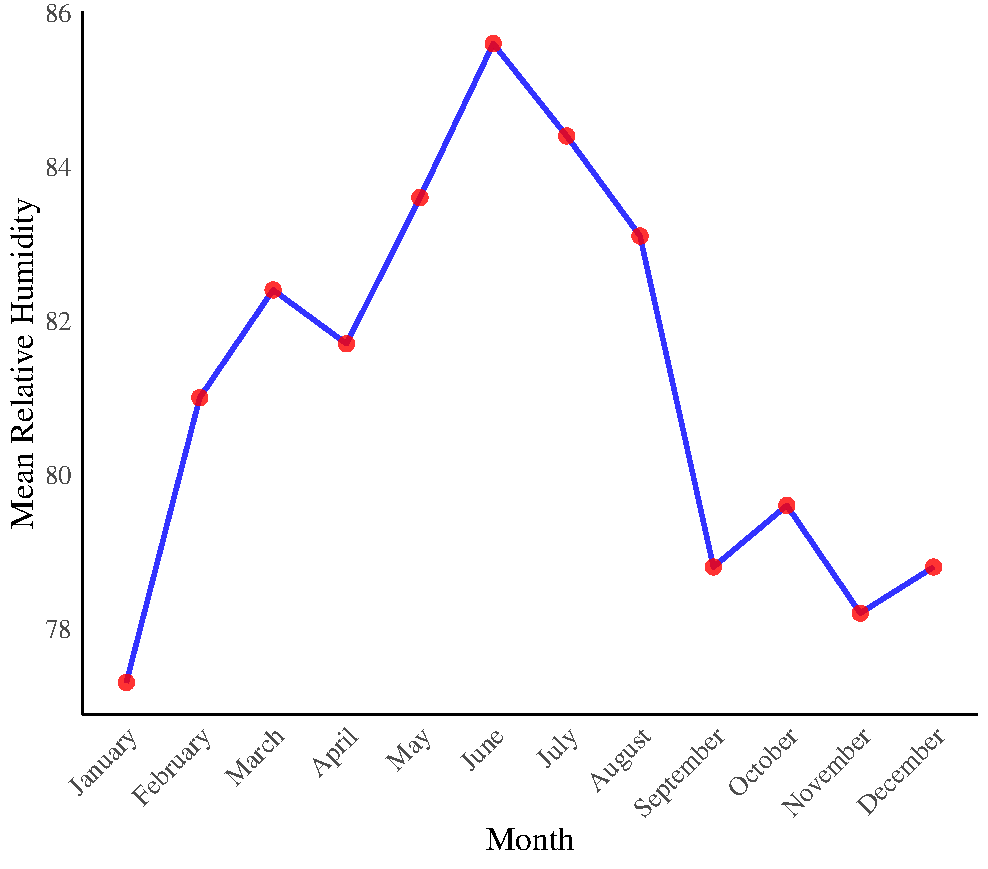
\includegraphics[width=0.6\textwidth]{humidity graph}
	\caption{Mean Monthly humidity in Wellington}
\end{figure}
%%% ACF Remove lines that carry no meaning

We construct the histogram of proportions $h=(h_1,h_2,h_3,h_4,h_5,h_6)$, where each bin $h_l$ represents the proportion of symbols of type $\pi^l$ out of the total six symbols. The histogram graph is shown below.

\begin{figure}
	\centering
	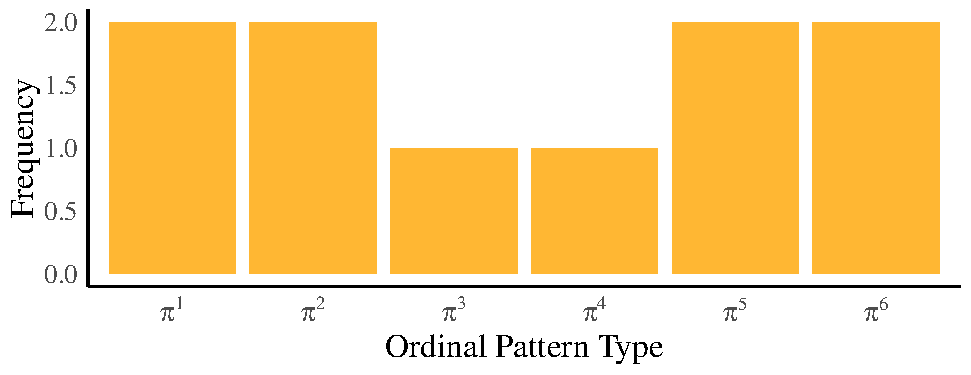
\includegraphics[width=0.6\textwidth]{frequency histogram}
	\caption{Histogram}
\end{figure}


\section*{Complexity Analysis in Time Series: Advantages and Limitations}

While this method effectively captures the ordinal relationships among data points, it has some drawbacks. Notably, it disregards the amplitude information of the time series. Additionally, in high-dimensional chaotic systems, classifying data using the complexity-entropy plane can be challenging or even misleading, as both high-dimensional deterministic time series and stochastic surrogate data may occupy similar regions in the plane.

Despite this limitation, integrating statistical complexity measures such as those derived from the complexity-entropy plane provides a powerful framework to complement ordinal pattern analysis. These measures quantify deviations from uniformity in the distribution of ordinal patterns, enabling a deeper characterization of the underlying dynamics. By combining permutation entropy with statistical complexity, researchers can more effectively distinguish between stochastic signals and deterministic chaos, offering a nuanced perspective on the structure and randomness of time series data.

\section*{The Bandt and Pompe Method: A Robust Approach}

The concept of ordinal patterns in time series can be effectively demonstrated through real world examples. Traditionally, numerous algorithms, techniques, and heuristics have been employed to estimate complexity measures from real world data. However, these methods often perform well only for low dimensional dynamical systems and struggle when noise is introduced.

The Bandt and Pompe method overcomes this limitation by providing a robust approach that remains reliable even in noisy environments. In time series analysis, key complexity measures such as entropy, fractal dimension, and Lyapunov exponents play a crucial role in comparing neighboring values and uncovering the underlying structure and dynamics of the data.

The advantages of Bandt \& Pompe methods:
\begin{itemize}
	\item Simplicity
	\item Extremely fast calculation
	\item Robutness
	\item Invariance to nonlinear monotonous transformations
\end{itemize}	

This method exhibits low sensitivity to noise and naturally accounts for the causal order of elements in a time series. As a result, it can be applied to various real-world problems, particularly in differentiating between chaotic and stochastic signals.

Despite its limitations, researchers have developed extensions to the original method to address its shortcomings and enhance its applicability to a broader range of complex systems.

\section*{Statistical Complexity measures}

After Bandt and Pompe introduced a successful method for analyzing time series, Rosso \cite{Rosso2007} expanded on this approach by incorporating statistical complexity derived from the same histogram of causal patterns. This method, which utilizes the complexity-entropy plane, has been successfully applied to various dynamic regimes including, system parameter change \cite{Cao2004,Bandt2005,Kowalski2007,Zunino2010a,Rosso2010a,Kowalski2011b,Zunino2012a, DeMicco2012a}, optical chaos \cite{Soriano2011a,Zunino2011a,Toomey2014,Yang2015e,Liu2016f}, hydrology \cite{Lange2013,Serinaldi2014,Stosic2016}, geophysics \cite{Consolini2014,Saco2010,Sippel2016}, engineering \cite{Yan2012,Aquino2015,Aquino2017,Redelico2017a}, biometrics \cite{Rosso2016}, characterization of pseudo-random number generators \cite{DeMicco2008,DeMicco2009}, biomedical signal analysis \cite{Zanin2012,Li2007,Li2008b,Parlitz2012,Morabito2012,Li2014b,Montani2014,Montani2014a,Liang2015b,Montani2015a,Montani2015}, econophysics \cite{Zanin2012,Zunino2010,Zunino2009, Bariviera2015a,Bariviera2015,Bariviera2016,Zunino2016a}.



 

However, despite the widespread use of ordinal patterns to study the latent dynamics of time series through permutation entropy, there are no established theoretical results concerning the distribution of permutation entropy that account for the correlation effects between patterns. Nonetheless, Rey et al. \cite{Rey2023a} demonstrated that the asymptotic distribution of permutation entropy is normal. They compared their findings with those of multinomial sample entropy, which assumes independence between patterns. Notably, the expression for the asymptotic variance becomes increasingly complex as the embedding dimension increases. 

This proposal has three objectives in order to continue this research work.
\begin{itemize}
	\item Define a data base of time series for clustering, i.e., finding similar time series. 
	\item Extract all the features we know from their Bandt \& Pompe symbolization (Shannon, Tsallis and Renyi entropies, Fisher information measure, complexities, and the available confidence intervals)
	\item Use those features for time series clustering 
\end{itemize} 




